\chapter{Theory}\label{cha:theory}
This chapter will discuss the theory behind \gls{ml} and \gls{fe}. We will briefly introduce a sketch of the steps in how the theory will be implemented, then describe the theory behind \gls{ml} and \gls{fe}, and then go into more detail about the different methods used in this project on the thoughts behind why choosing them.

\section{Images}\label{sec:images}
% As mentioned before, the project will use the \gls{mnist} dataset; the dataset comprises images; therefore, a digital image consists of pixels. In a grayscale image, each pixel has a value between 0 and 255, where 0 is white, and 255 is black. In a color image, each pixel has three values - one for each color: red, green, and blue; the amount of pixels in a color picture is the same as in a grayscale picture. A 28x28x1 grayscale image has 784 pixels, while a 28x28x3 color image also has 784 pixels~\cite{picture}.

% In this project, dimensionality reduction is shown by each pixel representing the image's feature (dimension). As the size of images increases, this quickly becomes a large number of features.

In this project there has been chosen to work with the \gls{mnist} dataset because it is commonly used in image recognition tasks, specifically for recognizing handwritten digits. This dataset is well-documented, which allows to compare the results to other similar projects, and it is small in size, making it easy to work with and not requiring a lot of computational power~\cite{lecun-mnist-database}.

It was considered to use the Iris and CIFAR-10 datasets, but the Iris dataset may have too few data samples ~\cite{mnist-vs-iris} and the CIFAR-10 dataset could be too complex for this project~\cite{datasets-uniqtech}. The \gls{mnist} dataset consists of images, and each image is composed of pixels. In a grayscale image, each pixel has a value between 0 and 255, with 0 representing white and 255 representing black~\cite{lecun-mnist-database}.

In this project aims to demonstrate dimensionality reduction by representing each pixel as a feature in the image. As the size of the images increases, this quickly becomes a large number of features.
% \subsection{Data}\label{sec:data}
% In this project, it was chosen to work with \gls{mnist}. \gls{mnist} was chosen because it has real-world uses inside image recognition, particularly recognizing handwritten numbers. The real-world use comes from detecting patterns in how numbers are written, which can be attributed to the writer's style, artificial errors, or both. 

% Another reason is that many projects revolve around recognizing handwritten digits using machine learning, therefore is well documented, which makes it easy to find information about it. That means this project can compare the results to similar projects for better discussion of results. The dataset is also tiny, which means it is easy to work with and does not require a lot of computing power~\cite{lecun-mnist-database}.

% The project could also have gone another route, such as collecting and cleaning data. However, choosing the \gls{mnist} dataset has simplified the overall work and allowed more focus on the project's machine learning/dimensionality reduction part. 

% The group has also considered the Iris dataset and the CIFAR-10 dataset. However, the Iris dataset might have too few data samples~\cite{mnist-vs-iris}, and the CIFAR-10 dataset would be too complex for this project~\cite{datasets-uniqtech}. Therefore the group has chosen to work with \gls{mnist}. As outlined before, there has been some preprocessing regarding the \gls{mnist}, which further solidified the choice of \gls{mnist}.




%which its creators describe as \textcquote{lecun-mnist-database}{The MNIST database of handwritten digits, available from this page, has a training set of 60,000 examples, and a test set of 10,000 examples. It is a subset of a larger set available from NIST. The digits have been size-normalized and centered in a fixed-size image}.

%Similarly, the digits in the dataset are \textcquote{lecun-mnist-database}{size-normalized and centered in a fixed-size image}, which means that Lecun et al.\ has worked with the data. 
\newacronym{relu}{ReLU}{Rectified Linear Unit}

\section{Machine Learning}\label{sec:machine-learning}
To determine the relevant dimensionality reduction methods to compare for the project, it is necessary to understand the basics of machine learning. This section describes the basics of machine learning and the different types of machine learning problems.


\subsection{Machine learning pipeline}\label{subsec:machine-learning-pipeline}
Figure~\ref{fig:basic-machine-learning-pipeline} shows the simplified and generalized steps in the pipeline of a machine learning model. The machine learning pipeline is divided into four main steps: data collection, feature engineering, model training and model evaluation.


\begin{figure}[htb!]
    \centering
    \begin{tikzpicture}
        \node (b) [state] {feature engineering};
        \node (c) [state, shift={($(b.east)+(2cm,0)$)}] {model};
        \node (a) [state, shift={($(b.west)+(-2cm,0)$)}] {data};
        \node (d) [state, shift={($(c.east)+(2cm,0)$)}] {evaluation};
        \node (e) [state, shift={($(b.south)+(0,-2cm)$)}] {parameters};

        \draw[arrow, ->] (a) -- node[above,scale=.70,align=center,] {} (b);
        \draw[arrow, ->] (b) -- node[above,scale=.70,align=center,] {} (c);
        \draw[arrow, ->] (c) -- node[above,scale=.70,align=center,] {} (d);
        \draw[arrow, ->] (e) -- node[above,scale=.70,align=center,] {} (c);

        \draw[arrow, ->] (d.north) -- ++(0,0.75) -| (b);
        \draw[arrow, ->] (d.south) -- ++(0,-0.75) -| (c);
    \end{tikzpicture}
    \caption{Simplified machine learning pipeline}
    \label{fig:basic-machine-learning-pipeline}
\end{figure}


The box with the name data represents the input to the machine learning pipeline. The data can be in different formats, such as images, text, audio, video, etc. The data is usually stored in a database or in a file. This is also the step where the data is cleaned and preprocessed.

Feature engineering represents the step where the data is transformed through dimensionality reduction. The reduced data is the input to the machine learning model.

Model training is the process of training the model with the data. This is done by splitting the data into a training set and a validation set. The training set is used to train the model to predict the output with highest possible accuracy. The validation set is used to evaluate the model, and may use cross validation to get a more accurate evaluation that avoids overfitting. The model depends on the type of machine learning problem.

Model evaluation represents the step where the model is evaluated. The evaluation is done by comparing the predictions of the model with the actual values. The evaluation is done on the validation set. The evaluation is done by using metrics such as accuracy, precision, recall, F1 score, etc. The evaluation is done to determine the performance of the model and to determine if the model is overfitting or underfitting.

The box with the name "parameters" represents the hyperparameters of the machine learning model. These parameters are set before training the model. The hyperparameters are usually set by the user, but can also be set by the machine learning model itself. The hyperparameters are usually set by trial and error, but there are also methods to find the best hyperparameters.

The arrows represent how machine learning models continously learn. The model is trained on the training set, and then evaluated on the validation set. The model is then updated with the new information, and the process is repeated. This is called the training loop. The training loop is repeated until the model converges, or until the model is no longer improving. The model is then evaluated on the test set, and the evaluation is used to determine the performance of the model.


\subsection{Data}\label{subsec:data}
Because the machine learning pipeline starts with the data, the choice of dataset for the project will impact all the following steps in the pipeline.

Most importantly the data must allow for the evaluation of the dimensionality reduction methods. Therefore, the dataset should be large enough dimensionally to perform meaningful dimensionality reduction. Furthermore, a well researched dataset is preferred, as it is more likely to be well suited for the evaluation of dimensionality reduction methods.

Based on the above requirements the \gls{mnist}~\cite{lecun-mnist-database} dataset is chosen. It is a dataset of images of 28x28 grayscale images of handwritten digits, making it well suited for the evaluation of dimensionality reduction methods, as the images are large enough to perform meaningful dimensionality reduction. Furthermore, the dataset is well researched, and has been used in many papers~\cite{lecun-mnist-database}.

In fact \gls{mnist} is so well researched that it may be considered overused~\cite{fashion-mnist}. If time permits, two similar datasets may be used in the project. The first is the \gls{fashion-mnist}~\cite{fashion-mnist} dataset, which is a variant of \gls{mnist} with images of clothing instead of handwritten digits. The second is the \gls{cifar}~\cite{krizhevsky-cifar} dataset, which consists of 50,000 training images and 10,000 test images of 32x32 color images of 10 different classes of objects.


\subsection{Feature engineering}\label{subsec:feature-engineering}
The theory deciding the choice of dimensionality reduction methods is described in Chapter~\ref{cha:theory}.

\todo[inline]{Some notes: normal distribution is relevant for LDA in particular apparently \url{https://www.rikvoorhaar.com/normal-data/}. FA is unlikely to be practical. PCA is the most common method}

\subsection{Machine learning models}\label{subsec:machine-learning-models}
Because \gls{mnist} is a set of labeled images, the machine learning problem is a multi-class classification supervised learning problem within the domain of computer vision, with the goal to train a model to predict the correct digit represented in an image.

Several machine learning models are used for image classification in general, and \gls{mnist} in particular~\cite{lecun-mnist-database,IBM-computer-vision,convolutional-neural-networks-convnets,multi-column-neural-network-ciregan}.

This project is not particularly concerned with the choice of machine learning model, but rather with the choice of dimensionality reduction methods. Therefore, \gls{svm} is chosen as the machine learning model. It is a relatively understandable model as it has similarities to the \gls{lda} method for dimensionality reduction \todo{perhaps better not to write this}, and has already been used with \gls{mnist} without dimensionality reduction~\cite{lecun-mnist-database}.

%why is there are the quora link.
% https://www.quora.com/What-is-the-difference-between-SVM-and-linear-discriminant-analysis

Additionally, a \gls{cnn} is used to compare the results of the dimensionality reduction methods with a more complex model. It is also used to compare the performance of the dimensionality reduction methods with a model that is not based on linear algebra. We will present what multi-class classification is, then explain how \gls{svm} and \gls{cnn} work.


\subsubsection{Multi-class classification}\label{subsubsec:multi-class-classification}
The \gls{mnist} dataset presents a multi-class classification problem, as the images can represent any of the 10 digits. The \gls{svm} model however is a binary classification model, and thus has to be adapted to the multi-class classification problem. There are two approaches to this problem: \gls{ovo} and \gls{ova}.

\gls{ovo} is a method where the model is trained on all possible combinations of two classes. For example, if there are 5 classes, the model is trained on 10 different models, one for each combination of two classes, this makes it computationally expensive as it has to go througth every combination. The model is then evaluated on all the models, and the class with the highest score is chosen as the predicted class.

\gls{ova} however is a method where the model is trained faster than in \gls{ovo}, as it only uses one class to distinguish if the data is similar or not. For example, if there are 5 classes, the model is trained on 5 different variations of the model, one for each class. This makes \gls{ova} good to distinguish between the current class that is being modeled from the other classes, however in \gls{ova} it is harder to distinguish between the other classes that is not being trained on. The model is then evaluated on all the models, and the class with the highest score is chosen as the predicted class~\cite{james-statistical-learning}.

\gls{ovo} is more computationally expensive than \gls{ova}, but is more accurate. The choice of \gls{ovo} or \gls{ova} is therefore a trade-off between accuracy and computational cost~\cite{james-statistical-learning}. The \gls{svm} model is chosen because it is a relatively simple model, and thus \gls{ova} is chosen as it is faster than \gls{ovo}.


\subsubsection{Support Vector Machine}\label{subsubsec:support-vector-machine}
\gls{svm} is a supervised learning model that classifies data by finding a mapping (hyperplane) that separates the classes in data~\cite{faster-svm}. \gls{svm} is also known as a large-margin classifier, which means that it relies on finding \textcquote{faster-svm}{a maximum-margin hyperplane to separate classes}. \gls{svm}, as the name implies, uses support vectors, are the 'vectors' that are closest to the function defining the mapping, and alterations on those data points will influence the hyperplane. For our purposes \gls{svm} is a promising model, since it is capable of defining a decision boundry which separates the classes the most. Such approach may be similar to how \gls{lda} works. An interesting property of \gls{svm} is that it can have among other parameters a kernel function, which can be tuned whether the data is linearly separable or not~\cite{faster-svm}. The kernel function that \gls{svm} shares resemblance to the way \gls{kpca} works, as it also uses a kernel function.


\subsubsection{Convolutional Neural Networks}\label{subsubsec:convolutional-neural-networks}
We assume that the reader is familiar with \gls{nn}s. The \gls{cnn}s are a specialized form of \gls{nn} that are mostly used for pattern recognition in images~\cite{introduction-to-cnn}. The reason we chose to work with \gls{cnn} is because, while normal \gls{nn}s are able to solve the classification problem regarding \gls{mnist}, they might not be as powerful as \gls{cnn}. The robustness of the \gls{cnn} can be shown in the sources~\cite{lecun-mnist-database, mnist-classification-benchmark}, where \gls{cnn}s are depicted as being 'state-of-the-art' machine learning models based on the minimum error rate that they achieve.


In our project it might not make a major difference, but using a \gls{cnn} can be better suited for image classifcation, as presented. Furthermore, according to Keiron et al.\ ~\cite{introduction-to-cnn}, \gls{nn}s are more prone to overfitting due to the layers being fully-connected, which increases the number of parameters, thereby increasing the complexity of the model. Another reason is the practicality / scalability of the model, as Keiron highlighted in his report, where he depicted a possible issue with \gls{nn}. The \gls{mnist} consists of $28 \times 28$ \textit{monochrome} pixels, which is relatively simple, compared to the real-world images which can be bigger, and have three colors / channels. We know that \gls{nn}s are fully-connected layers, in essence, neurons are connected to all the neurons in the previous layer, and Figure \ref{fig:nn-example-architecture} can provide a visual aid. When the amount of pixels is large, and colorized, then so should the size of the \gls{nn} be~\cite{introduction-to-cnn}.

\begin{figure}[htb!]
    \centering
    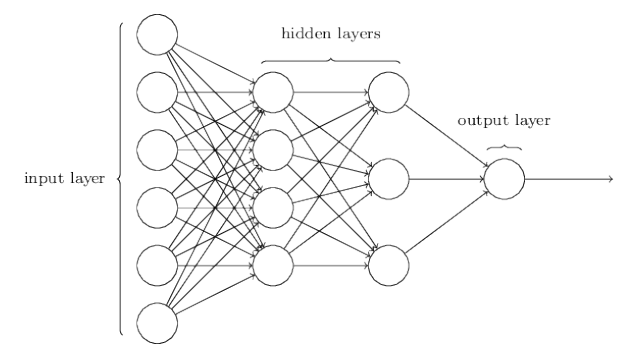
\includegraphics[width=0.65\textwidth]{figures/michael-nielsen-nn-architecture.png}
    \caption{An example of a neural network architecture~\cite{michael-nielsen-nn}}
    \label{fig:nn-example-architecture}
\end{figure}

The difference between \gls{nn} and \gls{cnn} is the among others the architectural blueprint. In \gls{cnn} neurons also have another property: the neurons are arranged in three dimensions: \textcquote{introduction-to-cnn}{the spatial dimensionality of the input(\textbf{height} and the \textbf{width}), and the \textbf{depth}}. The spatial dimensionality is the pixels, and the depth is one, since \gls{mnist} is monochrome.


%Ugly figure and not 100% visual, but it is simple
\begin{figure}[htb!]
    \centering
    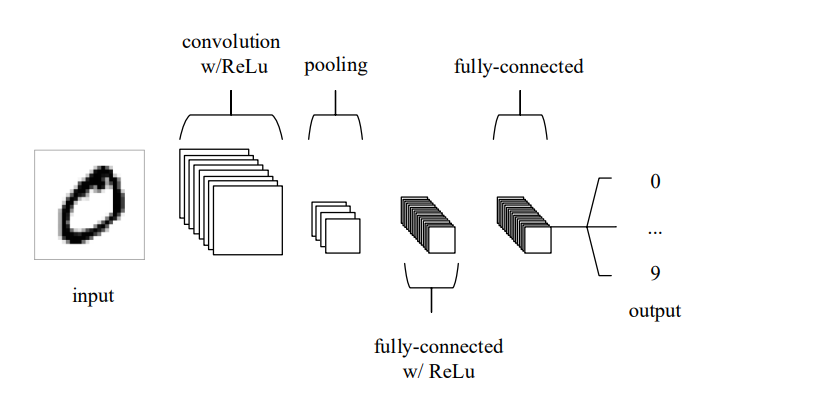
\includegraphics[width=0.8\textwidth]{figures/cnn-simple-architecture.png}
    \caption{An example of a convolutional neural network architecture~\cite{introduction-to-cnn}}
    \label{fig:simple-cnn-architecture}
\end{figure}
%Blog-like structure where CNN is depicted

\gls{cnn}'s architecture constitutes three different types of layers: convolutional layers, pooling layers, and fully-connected layers. The architecture of a \gls{cnn} can be shown in Figure \ref{fig:simple-cnn-architecture}. The convolutional layers \textcquote{introduction-to-cnn}{will determine the output of neurons of which are connected to local regions of the input}, which is also called a convolution. The pooling layers reduce the number of parameters in the previous layers. The fully-connected layers act as normal \gls{nn} layers~\cite{introduction-to-cnn}.


A convolution, as described, acts as a filter which maps the input to an output matrix $conv$ of size $n \times n$. The mapping is done by the elementwise-multiplication of the input matrix with the $conv$ matrix. The operation can be seen in Figure \ref{fig:convolution}. The manner in which such mapping is achieved is by sliding over the input matrix, from left to right, top to bottom, with a $n \times n$ matrix one pixel at a time. For each convolution operation \gls{relu} is applied to the operation, where \gls{relu} is a function which takes the maximum value between 0 and the input~\cite{google-cnn}.

\begin{figure}[htb!]
    \centering
    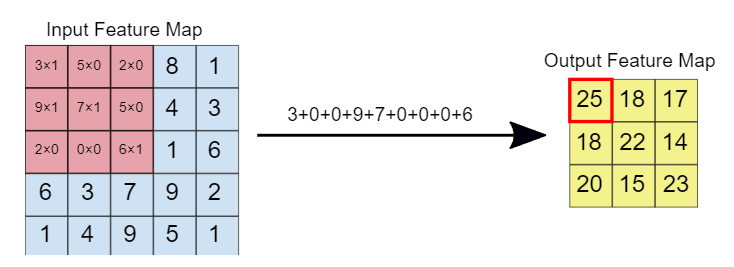
\includegraphics[width=0.7\textwidth]{figures/google-cnn-convolution-example.png}
    \caption{An example of a convolution operation~\cite{google-cnn}}
    \label{fig:convolution}
\end{figure}

In the pooling layer behaves like a convolution, but this time it filters the $conv$ matrix with a $pool$ matrix of size $n \times n$. One method which has been presented~\cite{google-cnn} is the use of max pooling; in the convolutional layer the elementwise multiplication is applied, whereas in max pooling the element with the highest number in the respective matrix is chosen~\cite{google-cnn}. Figure \ref{fig:maxpooling} is provided to show how it works. The pooling layer can be seen as a dimensionality reduction method, because it reduces the data while preserving the original features.

\begin{figure}[htb!]
    \centering
    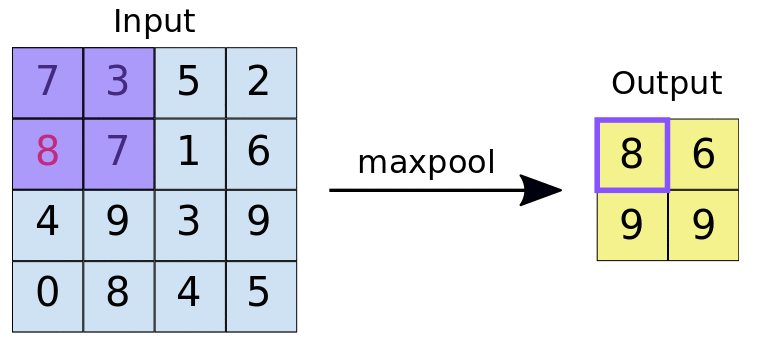
\includegraphics[width=0.5\textwidth]{figures/google-cnn-maxpooling-example.png}
    \caption{An example of a max pooling operation~\cite{google-cnn}}
    \label{fig:maxpooling}
\end{figure}

The last layer is the fully-connected layer, which is connected to all the neurons from the pooling layer. According to Keiron ~\cite{introduction-to-cnn}, the activation function \gls{relu} might be suited to be used in this layer too~\cite{lecun-mnist-database}.

\subsection{Model training}\label{subsec:model-training}
The theory deciding the cross validation methods is described in Chapter~\ref{cha:theory}.



% @book{michael-nielsen-nn,
%   title={Neural networks and deep learning},
%   author={Nielsen, Michael A},
%   volume={25},
%   year={2015},
%   publisher={Determination press San Francisco, CA, USA}
% }
% @misc{faster-svm,
%   doi = {10.48550/ARXIV.1808.06394},
  
%   url = {https://arxiv.org/abs/1808.06394},
  
%   author = {Schlag, Sebastian and Schmitt, Matthias and Schulz, Christian},
  
%   title = {Faster Support Vector Machines},
  
%   publisher = {arXiv},
  
%   year = {2018},
  
%   copyright = {arXiv.org perpetual, non-exclusive license}
% }


% @misc{introduction-to-cnn,
%   doi = {10.48550/ARXIV.1511.08458},
  
%   url = {https://arxiv.org/abs/1511.08458},
  
%   author = {O'Shea, Keiron and Nash, Ryan},
  
%   title = {An Introduction to Convolutional Neural Networks},
  
%   publisher = {arXiv},
  
%   year = {2015},
  
%   copyright = {arXiv.org perpetual, non-exclusive license}
% }


% @misc{mnist-classification-benchmark,
%     url = {https://paperswithcode.com/sota/image-classification-on-mnist},
%     title = {Image Classifcation onf MNIST},
%     year = {2022}
% }

% @misc{google-cnn,
%     organization = {Google},
%     url = {https://developers.google.com/machine-learning/practica/image-classification/convolutional-neural-networks},
%     title = {ML Practicum: Image Classification},
%     year = {2022}
% }

\section{Classification}\label{sec:classification}
When making a model, it is only sometimes possible to predict the value of a variable. For example, if one wants to predict a house's price, one can not predict the exact price, but may be able to predict if the price is high or low. This is called classification. In \gls{ml}, classification is when a quantitative answer is not required; a qualitative answer is satisfying. The goal is to classify the input into one of a set of categories set in the dataset. As long as the dataset supports supervised learning, classification can be applied to it~\cite{james-statistical-learning1}.
This is done by training a model on a labeled dataset and then using the model to predict the category of new, unlabeled data~\cite{james-statistical-learning1}.

The training data consists of input and class label pairs. The input can be a single value, such as numbers or strings, or vectors of values, such as a list of numbers or strings. The input can also be a matrix of values, such as a grayscale or color image. The class label is a discrete value, such as a number or a string. In this project, a class label is a number representing the digit in the image~\cite{james-statistical-learning1}.

The model is trained to minimize the error between the predicted and actual class labels. The error is calculated by comparing the predicted class label with the actual class label~\cite{james-statistical-learning1}.

The model is trained by finding the best parameters for the model, such as weights in a neural network or parameters in models, such as \gls{svm}~\cite{james-statistical-learning1}. These parameters help the model predict the category of new data. Hyperparameter optimization is finding the best parameters; this is discussed further in Section~\ref{sec:hyperparam}.

One must consider the data and the problem when deciding which model to use. The model must be able to handle the data and the problem. In this project, the \gls{ml} model is used for image classification, as the \gls{mnist} dataset is used. Several \gls{ml} models have been used for image classification with \gls{mnist} in general; the ones the group has looked into is~\cite{lecun-mnist-database,IBM-computer-vision,convolutional-neural-networks-convnets,multi-column-neural-network-ciregan}. These models can be used to classify images into one of ten categories, representing the digits 0-9, as this is the project's focus.

\subsubsection{Support Vector Machine}\label{subsubsec:support-vector-machine}
\gls{svm} is a supervised \gls{ml} model that can be used for classification or regression problems. It is a linear model for classification and regression problems. It is a binary classifier, meaning it can only classify two classes. It is a linear classifier, meaning it makes a decision based on a linear function of the input features~\cite{james-statistical-learning1}.

\gls{svm} classifies data by finding a mapping (hyperplane) that separates the classes in data~\cite{faster-svm}. \gls{svm} is also known as a large-margin classifier, which means that it relies on finding \textcquote{faster-svm}{a maximum-margin hyperplane to separate classes}. As the name implies, \gls{svm} uses support vectors, which are the 'vectors' closest to the function defining the mapping, and alterations on those data points will influence the hyperplane.
An exciting property of \gls{svm} is that it can have, among other parameters, a kernel function, which can be tuned whether the data is linearly separable or not~\cite{faster-svm}. The kernel function that \gls{svm} resembles the way \gls{kpca} works, as it also uses a kernel function.

For the project's purposes, \gls{svm} is a promising model since \textcquote{james-statistical-learning1}{SVMs have been shown to perform well in a variety of settings and are often considered one of the best "out of the box" classifiers.}. This is because \gls{svm} is a linear model, which means it is fast to train and predict. This is important for the project, as the model needs to classify the images quickly. The model also has a high accuracy, which is vital for the project, as the model needs to classify the images correctly. Though it is not as accurate as other models, such as \gls{nn}, it is still a good model for the project. On the downside of \gls{svm}, ~\cite{james-statistical-learning1} states \textcquote{james-statistical-learning1}{Though it is elegant and simple, we will see that this classifier, unfortunately, cannot be applied to most data sets, since it requires that the classes be separable by a linear boundary}. It means there can be some errors in the \gls{ml} model, as it is only sometimes possible to separate the classes in \gls{mnist} by a linear boundary; this is something the group has considered choosing the model.

This project is not mainly concerned with the choice of \gls{ml} model but rather with the choice of dimensionality reduction methods. Therefore, \gls{svm} is chosen as the \gls{ml} model as it has already been used with \gls{mnist} without dimensionality reduction~\cite{lecun-mnist-database}.



\subsection{Multi-class classification}\label{subsec:multi-class}
In classification, there are two types of classification, binary classification, and multi-class classification. Binary classification is the classification of two classes, while multi-class classification is the classification of more than two classes. The \gls{mnist} dataset used in this project presents a multi-class classification problem, as the images can represent any of the ten digits. The \gls{svm} model, however, is a binary classification model and thus has to be adapted to the multi-class classification problem. there will explained two approaches to this problem: \gls{ovo} and \gls{ova}~\cite{james-statistical-learning1}.

\subsubsection{One-vs-One}\label{subsubsec:one-vs-one}
\gls{ovo} is a method where the model trains on all possible combinations of two classes. For example, if there are five classes, the model is trained on ten different models, one for each combination of two classes; this makes it computationally expensive as it has to go through every combination. Then the model is evaluated against all other models, and the class with the highest score is picked as the predicted class~\cite{james-statistical-learning1}.

\subsubsection{One-vs-All}\label{subsubsec:one-vs-all}
However, \gls{ova} is faster than \gls{ovo}, as it only uses one class to distinguish if the data is similar. For example, if there are five classes, the model is trained on five variations of the model, one for each class. This makes \gls{ova} good to distinguish between the current class that is being modeled from the other classes. However, in OVA, it is harder to distinguish between the other classes that are not being trained. Then the model is then evaluated on all models, and the class with the highest score is chosen as the predicted class~\cite{james-statistical-learning1}.

\subsubsection{One-vs-One vs One-vs-All}\label{subsubsec:one-vs-one-vs-one-vs-all}
\gls{ovo} is more computationally expensive than \gls{ova}, but is more accurate. The choice of \gls{ovo} or \gls{ova} is, therefore, a trade-off between accuracy and computational cost~\cite{james-statistical-learning1}. \gls{ovo} is chosen as the method for multi-class classification. \todo[inline]{We use OvO because it is faster than OvA, make that clear.}

\section{Preprocessing}
In this section, the theory of preprocessing and what effects it has on the \gls{ml} model is discussed. 

%What is preproccessing?
%What effects does it have on the model/data?
%Why do we need it?
%What are the steps?
%What are the tools?
%What are the results?

\subsection{Definition of preproccessing}\label{subsec:preprocessing-definition}
The proper definition of preproccessing or data preparation, varies depending on the source. The definition that will be used in this report, is given as:
\textcquote{doi:10.1080/713827180}{Data preparation comprises those techniques concerned with analyzing raw data so as to yield quality data, mainly including data collecting, data integration, data transformation, data cleaning, data reduction, and data discretization.}
From this, it can be gathered that preproccessing is a broad term, which can be divided into several subcategories. Not all subcategories will be relevant for this project, therefore only relevant subcategories of preprocessing will be discussed in the following sections.

\subsection{Reasons for preproccessing}
As stated in the definition, preproccessing is used, among other reasons, to yield quality data. The importance of this, stems from the fact that real world data, is not always clean or complete. Meaning that can be a lot of noise, which is data that either contains errors or outliers. This noise can be removed by preproccessing, which creates a more accurate, higher quality, and smaller dataset, to gather information from. This results in a reduced amount of data that the model is trained on, but the data it is trained on, should be more accurate, which should then train the model more accurately and efficiently \cite{doi:10.1080/713827180}.

Data collected, may be in a form or shape that is not compatible with the process that is needed to work with it, therefore in order to use the data, it may need to be transformed into a form that is compatible with the process. Transformation of data, can be many things, as \cite{Data-preprocessing-for-flight-delays} mentions normalization as a part of transformation, to scale the data so that it fits into a new range, a more detailed explanation of normalization will be given in \ref{sec:normalization}.


\subsection{Steps of preproccessing}
The amount of preproccessing, depends on what is needed, and what is available. An example of how these steps could be used, can be seen in the report \cite{Data-preprocessing-for-flight-delays}. Where they start by cleaning data, then transform it, then reduce it, and finally balance it. For this section, the theory of the steps that are used in this report, will be explained.

\subsubsection{Reshape}
The data, when loaded in at first, is shaped as a long array of 47.040.000 integers, that represent the values of the pixels, and then another array of 60.000 integers, that represents what number, a given image is. The images, are to be thought of as a 28x28 matrix, meaning that the first 784 integers, represent the first image, and the next 784 integers represent the second image. Working with the data in this format, proved difficult and confusing, as it was hard to keep track of what image was being worked on. Because of this, it was decided to reshape the data, to make it easier to understand. The data was reshaped to a 2 dimensional array, where the first dimension represented the array of images, and the second dimension represented the array of pixels and their values. From this, there was a clear distinction between each image.

An example, to further explain the decision for reshaping the data, can be seen in \cite{scikit-learn-PCA}, where it is stated that the function \texttt{fit} expects: \textcquote{scikit-learn-PCA}{X : array-like of shape (n\_samples, n\_features)}. Meaning that data is expected to be sectioned into an array of samples(images), and an array of features. When the data was not reshaped, it was not possible to use the \texttt{fit} function, as the data was not in the correct format. The data would have a n\_samples, that was of the size 47.040.000, which is not the actual number of samples (images), but rather the number of pixels that exist in all 60.000 images.

\section{Normalization}\label{sec:normalization}
Scaling, also called feature normalization, is the process of transforming the data into a form that is more suitable for the \gls{ml} model. This is done by changing the range of the data, for example, if the data is in the range of 0-100, it can be scaled to be in the range of 0-1. This is done to make the data more suitable for the model, and to make it easier to compare the data. Scaling is also a standard practice in most machine learning problems. There are many ways to scale the data, one way is to use the min-max scaler, another way is to use variance scaling~\cite{Feature-engineering-zheng}.
\subsection{Min-max scaler}
The min-max scaler is a simple way to scale the data. It scales the data to be in the range of 0-1. The formula for the min-max scaler is:
\begin{equation}
    x_{scaled} = \frac{x - x_{min}}{x_{max} - x_{min}}
\end{equation}
where $x$ is the original value, $x_{scaled}$ is the scaled value, $x_{min}$ is the minimum value in the data, and $x_{max}$ is the maximum value in the data. The min-max scaler is a simple way to scale the data, but it is not robust to outliers. If there are outliers in the data, the min-max scaler will scale the data to be in the range of 0-1, but the outliers will be scaled to be very close to 0 or 1. This can be a problem if the outliers are important to the model. The min-max scaler is also sensitive to the presence of zeros in the data. If there are zeros in the data, the min-max scaler will scale the data to be in the range of 0-1, but the zeros will be scaled to be 0. This can be a problem if the zeros are important to the model. 



% @misc{scikit-learn-PCA,
%   year  = {2022},
%   month = {Nov 22},
%   title = {sklearn.decomposition.PCA},
%   url   = {https://scikit-learn.org/stable/modules/generated/sklearn.decomposition.PCA.html#sklearn.decomposition.PCA.fit}
% }

% @article{doi:10.1080/713827180,
%     author = { Shichao   Zhang  and  Chengqi   Zhang  and  Qiang   Yang },
%     title = {Data preparation for data mining},
%     journal = {Applied Artificial Intelligence},
%     volume = {17},
%     number = {5-6},
%     pages = {375-381},
%     year  = {2003},
%     publisher = {Taylor & Francis},
%     doi = {10.1080/713827180},
%     URL = {https://doi.org/10.1080/713827180},
%     eprint = {https://doi.org/10.1080/713827180}
% }

% @INPROCEEDINGS{Data-preprocessing-for-flight-delays,
%     author={Moreira, Leonardo and Dantas, Christofer and Oliveira, Leonardo and Soares, Jorge and Ogasawara, Eduardo},  booktitle={2018 International Joint Conference on Neural Networks (IJCNN)},   title={On Evaluating Data Preprocessing Methods for Machine Learning Models for Flight Delays},
%     year={2018},
%     volume={},
%     number={},
%     pages={1-8},
%     doi={10.1109/IJCNN.2018.8489294},
% }



%Explain why this is needed, for other reasons than just making it easier to understand.
%Does scikit methods need it to be in this format?
%Easier to use a function on a single image 

%Reshape
%normalize/Scale - StandardScaler
    %Look at others



%focus on cleaning or dim reduction
%Is augmentation a part of preproccessing?
%What is the difference between cleaning and dim reduction?
%Transforming data to fit our current needs
%






%Data preparation comprises those techniques concerned with analyzing raw data so as to yield quality data, mainly including data collecting, data integration, data transformation, data cleaning, data reduction, and data discretization.
    %We want data preprocessing, due to real world data being incomplete, noisy, and inconsistent.
    %Generates a smaller dataset to work with, which makes it more efficient for datamining.


%https://www.frontiersin.org/articles/10.3389/fbioe.2020.00260/full
    %Data preprocessing subcategories: (1) Ground reaction force (GRF) filtering, (2) time derivative, (3) time normalization, (4) data reduction, (5) weight normalization, and (6) data scaling.

%https://praveenkds.medium.com/data-preparation-for-machine-learning-data-cleaning-data-transformation-data-reduction-c4c86c4471a1
    %Data cleaning: removing noise, outliers, and missing values.
    %Data transformation: scaling, normalization, and discretization.
    %Data reduction: feature selection and feature extraction.
\section{Dimensionality reduction}\label{sec:dimensionality-reduction}
In general, dimensionality reduction transforms data with many features (dimensions) into a new representation of the data with fewer features while preserving as much relevant information as possible. Dimensionality reduction is made by finding a transformation of the data that maps the data to some lower dimensional space while keeping the mean distances between the data points~\cite{dimensionality-reduction-comparative-review}.

Dimensionality reduction can be divided into two categories: linear and nonlinear methods, described in Section \ref{sec:linear-vs-nonlinear}. This section presents some of the standard methods from both categories.

\todo[inline]{Linear methods are based on the assumption that the data is linear. 
A linear dataset is one in which all possible prediction outcomes can be obtained by combinations of the original features without any additional interactions. 
You can show an example of linear data for regression and classification. 
Note that this difference is not so strict as some methods could be thought of as both}


\subsection{Linear methods}\label{subsec:linear-methods}
The linear methods covered are: \gls{pca}, \gls{fa}, \gls{nmf}, and \gls{lda}.


\subsubsection{Principal Components Analysis}\label{subsubsec:principal-components-analysis}
\gls{pca} is a linear method used to reduce a dataset's dimensionality by projecting it onto a lower dimensional subspace, retaining as much of the variance as possible. The best projection is found through the directions of maximum variance in the data based on the covariance matrix and then projecting the data onto those directions. The directions of maximum variance are principal components, and the projection results from the \gls{pca}~\cite{dimensionality-reduction-comparative-review}.


\subsubsection{Factor Analysis}\label{subsubsec:factor-analysis}
\gls{fa} is very similar to \gls{pca}, and \gls{pca} may be called a type of \gls{fa}. However, \gls{fa} is based on the assumption that the data is generated by a linear combination of a few latent variables called factors and that the observed variables are a linear combination of the latent variables plus some noise.

The goal of \gls{fa} is to find the factors that explain the most covariance in the data. Intuitively, related items have stronger mathematical correlations and can thus be grouped with less loss of information. Once the correlations are determined, a rotation is performed to make the factors easier to interpret~\gls{fa}~\cite{decoster-1998-factor-analysis-overview}.


\subsubsection{Non-negative matrix factorization}\label{subsubsec:non-negative-matrix-factorization}
\gls{nmf} constructs approximate factorizations of a non-negative data matrix $V$ into two non-negative matrices $W$ and $H$ such that $V \approx WH$. The non-negativity constraints permit the intuition that data may represent parts forming a whole, which can be thought of as a sum of parts~\cite{lee-1999-learning-nmf}. For example, a text document may represent a combination of topics, and each may represent a combination of words.


\subsubsection{Linear Discriminant Analysis}\label{subsubsec:linear-discriminant-analysis}

\gls{lda} is quite similar to \gls{pca} since they both try to project data into a hyperplane. Still, instead, \gls{lda} tries to maximize class separability, making it easier to contrast classes. \gls{lda} finds the hyperplane with the most separation between the classes and keeps the data points with the same class as close together as possible. This is a three-step process. The first step is to determine the separation between different classes (between-class variance) as the distance between the means of each class. Secondly, the distance between the mean and samples of each class (within-class variance) is calculated. The third step is creating a lower dimensional representation that maximizes the between-class variance and minimizes the within-class variance~\cite{linear-discriminant-analysis-tutorial}.


\subsection{Non-linear methods}\label{subsec:non-linear-methods}
Sometimes high-dimensional data may contain non-linear relationships, which linear methods cannot capture. It has been shown that \gls{pca} fails to find significant components in the swiss-roll dataset~\cite{tennenbaum}. In such cases, non-linear methods are used. The non-linear methods covered are \gls{kpca}, \gls{mds}, and \gls{isomap}.


\subsubsection{Kernel Principal Component Analysis}\label{subsubsec:kernel-principal-component-analysis}
\gls{kpca} is an extension of \gls{pca}, and it projects the data onto a higher dimensional plane, where \gls{pca} is performed. 
The first step is to construct the kernel matrix from the data. The kernel matrix is a matrix of the dot products of the data points, the kernel matrix is used like the covariance matrix in \gls{pca}~\cite{kernel-pca}. In the kernel matrix the data is in a higher dimensional space, where the data is linear separable. By using the kernel function, \gls{kpca} exposes the kernel trick, which is instead of calculating the dat into a higher dimensional space, it calculates the inner product between the datapoints, which is computationally cheap to calculate instead of calculating every datapoint into a higher dimensional space.
The kernel matrix is then centered by subtracting the mean of each row and column. This matrix is also called the Gram matrix. The Gram matrix is then used to find eigenvectors and eigenvalues. By using the kernel trick, \gls{kpca} can compute eigenvalue decomposition, as in \gls{pca}.The eigenvectors are then used to project the data onto a higher dimensional space, where \gls{pca} is performed. The eigenvectors with the highest eigenvalues are the principal components, and the projection is the data projected onto the principal components~\cite{kernel-pca}. 

\subsubsection{Isometric Feature Mapping}\label{subsubsec:isometric-feature-mapping}
\gls{isomap} is another non-linear method that is a special case of \gls{cmds}. It is assumed that \gls{isomap} is suited to discover manifolds of arbitrary dimensionality and that it guarantees an approximation of the true structure of the manifold~\cite{tennenbaum}.

The first step in \gls{isomap} is to map the data points in a graph. The graph is constructed by connecting each point to its nearest neighbors. The user sets the number of nearest neighbors. The nearest neighbors are found by using the Euclidean distance. The Euclidean distance is the linear distance between two points in a Euclidean space~\cite{Multidimensional-Scaling-Sammon-Mapping-and-Isomap}.

In the second step, \gls{isomap} finds the Geodesic distance between each point~\cite{Multidimensional-Scaling-Sammon-Mapping-and-Isomap}. The Geodesic distance is the shortest distance between two points on the surface of a sphere. The Geodesic distance is calculated by finding the shortest path between two points on a graph. The graph is constructed by connecting each point to its nearest neighbors. The shortest path can be found by using the Dijkstra algorithm~\cite{multi-dimensional-scaling-leeuw}.

The final step in \gls{isomap} is finding the data's \gls{mds} projection. The \gls{mds} projection is found by minimizing the stress function. The stress function is the sum of the squared differences between the distances in the original data and the distances in the projected data~\cite{multi-dimensional-scaling-leeuw}, so the stress function finds the slightest change in the data. The minimum of this stress function will be the best reproduction of the data in lower dimensional space according to the \gls{isomap} algorithm. 



\subsection{Choice of dimensionality reduction}
Four different dimensionality reduction methods have been chosen to be in the implementation. These are linear and nonlinear methods, particularly \gls{pca}, \gls{lda}, \gls{kpca}, and \gls{isomap}. The group chose these four because they cover the spectrum of options well and are some of the most used. Only four were selected to keep the project's focus tight and the right amount of depth versus breadth of the project.

%ISOMAP 


%The geodesic distance is used in \gls{isomap} to find the shortest distance between two points in a dataset. %These will be clarified first before clarifying \gls{isomap}. 

%\subparagraph{Multi Dimensional Scaling}\label{subsec:multi-dimensional-scaling}
%\gls{mds} is a non-linear method that is used to reduce the dimensionality of a dataset by projecting it onto a lower dimensional subspace, while preserving as much of the variance between the data as possible. The projection is found by calculating the best result from the \gls{mds} function which is a modified version of the STRESS function. The STRESS function finds the least change in data when in the case of \gls{mds} is when reducing the dimensionality~\cite{multi-dimensional-scaling-leeuw}.

%\subparagraph{Geodesic distance}\label{subsec:geodesic-distance}
%Geodesic is a distance between two points on a surface of a sphere. The geodesic distance between two points is the shortest distance between the two points on the surface of a sphere. The geodesic distance is calculated by finding the shortest path between two points on a graph. The graph is constructed by connecting each point to its nearest neighbors. The shortest path is found by using the Dijkstra's algorithm~\cite{multi-dimensional-scaling-leeuw}.


% In this project we will focus on dimensionality reduction for the purpose of computer vision, and in particular for the MNIST dataset.


% In this project we will study some common methods of dimensionality reduction using the MNIST dataset for digit recognition.
\section{Examples of methods}\label{sec:examples-methods}
In this section we will present how the linear and nonlinear methods behave on linear and nonlinear data. It should be noted again that the methods have different purposes. As a quick reminder \gls{pca} tries to maximize the variance in the embedded data (and so does \gls{kpca}), while \gls{lda} tries to maximize the separability of classes in the data, and \gls{isomap} tries to preserve the distances from the high-dimensional data when projecting it onto a lower space. Therefore their results will not a one-to-one comparison.


\subsection{Linear data example}\label{subsec:linear-data-example}
As linear data we will use the Iris dataset, which contains three different species of Iris flowers, with 50 examples each. Each class has four dimensions, which are the length and width of the sepals, and petals ~\cite{iris-dataset}. The dataset is a simple and well-known dataset, which has been used in many machine learning papers ~\cite{iris-dataset}, and should give intuition as to how the methods behave on the dataset.

\begin{figure}[htb!]
\centering
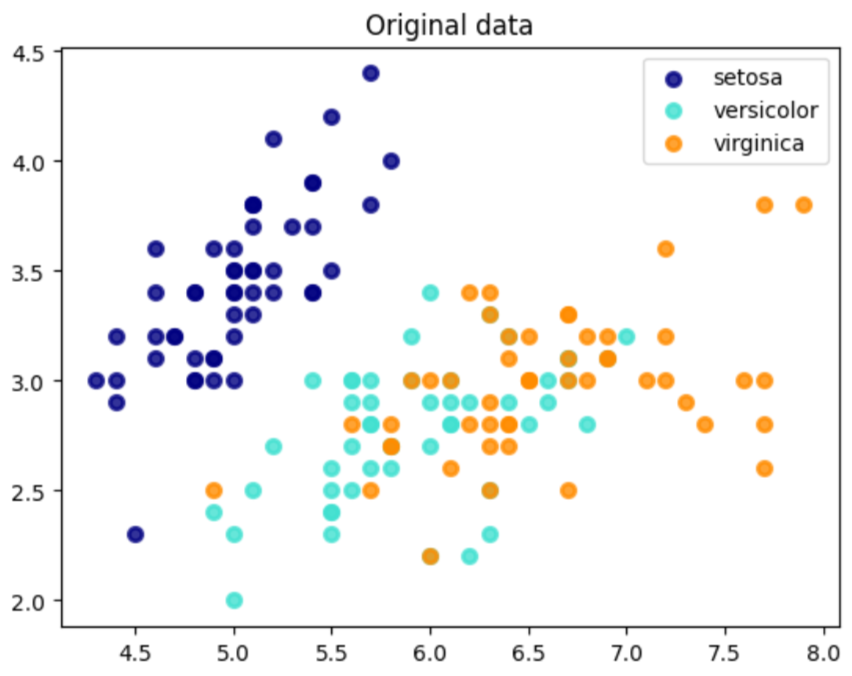
\includegraphics[width=0.5\textwidth]{figures/theory-example-figures/linear-data.png}
\caption{Linear data as Iris dataset}
\label{fig:linear-data}
\end{figure}

On figure \ref{fig:linear-data} the iris flowers are represented on a 2D plot. According to ~\cite{iris-dataset} only one class is separable, and that can further be  solidified by the fact that the species setosa is the only class that is visually linearly separable.

\subsubsection{Linear methods}\label{subsubsec:linear-methods-on-iris}
On figure \ref{fig:iris-pca} one can see that \gls{pca} has successfully separated the setosa species from the other classes in the dataset. With respect to the other species, on the coordiantes [1.20, 0.20] they do not seem to be clearly separated.

\begin{figure}[htb!]
\centering
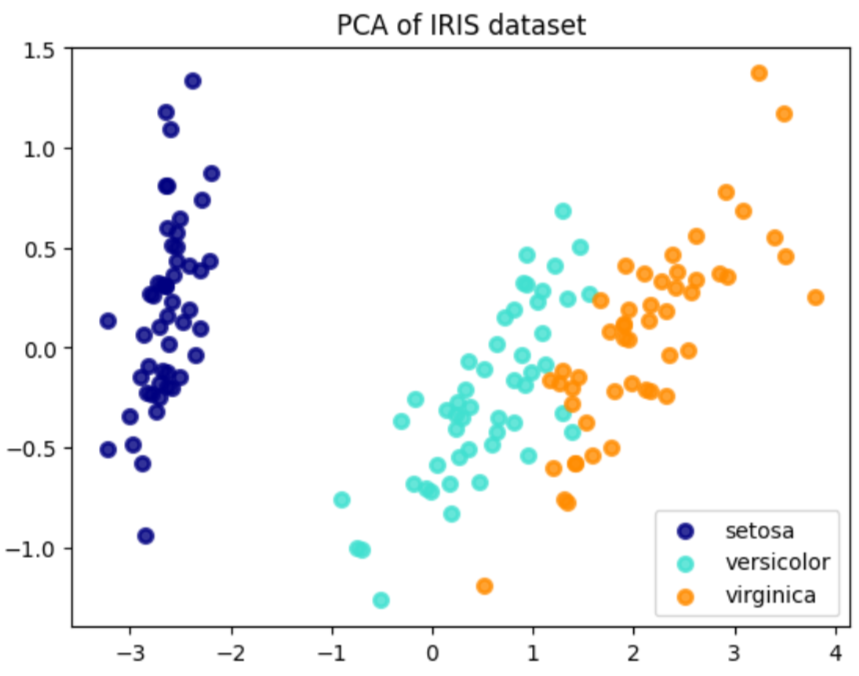
\includegraphics[width=0.5\textwidth]{figures/theory-example-figures/iris-pca.png}
\caption{PCA on iris}
\label{fig:iris-pca}
\end{figure}


\begin{figure}[htb!]
    \centering
    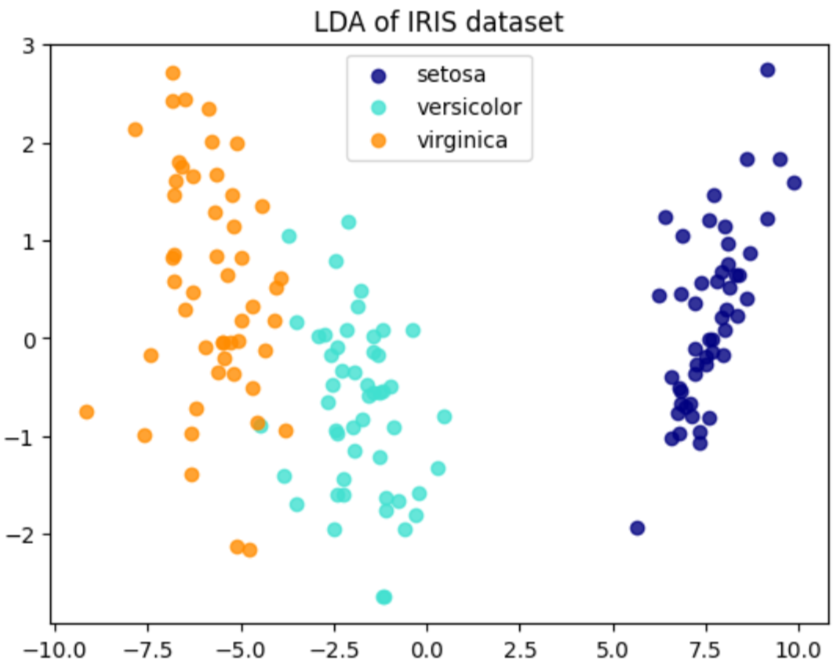
\includegraphics[width=0.5\textwidth]{figures/theory-example-figures/iris-lda.png}
    \caption{LDA on iris}
    \label{fig:iris-lda}
    \end{figure}
    
On figure \ref{fig:iris-lda} \gls{lda} has also successfully separated the setosa species from the other classes in the dataset. In contrast with \gls{pca}, \gls{lda} has managed to separate somewhat better as the distinction between those classes can be made easier. An advantage, which \gls{lda} poses, is that \gls{lda} is a supervised method, which means that LDA knows the labels of the data, and therefore may be better suited for classifying the data.

\subsubsection{Nonlinear methods}\label{subsubsec:nonlinear-methods-on-iris}
On figure \ref{fig:iris-isomap} \gls{isomap} has tried to separate the setosa, and managed to map the data on the first two dimensions. \gls{isomap}, as opposed to the aforementioned linear methods, has not found too much diversity on the second projection, as the values range from approximative 0.0 to -0.25. Such range is short in comparison with the linear methods. Isomap clusters the setosa species, but that may not be helpful if the data needs to be projected on two dimensions. If, for example, a point is in upper left corner, then it is not possible to tell if it is a setosa, or a versicolor. \gls{isomap} is nevertheless a nonlinear method, and it is expected that it does not reduce the data as efficiently as the linear methods do.

\begin{figure}[htb!]
    \centering
    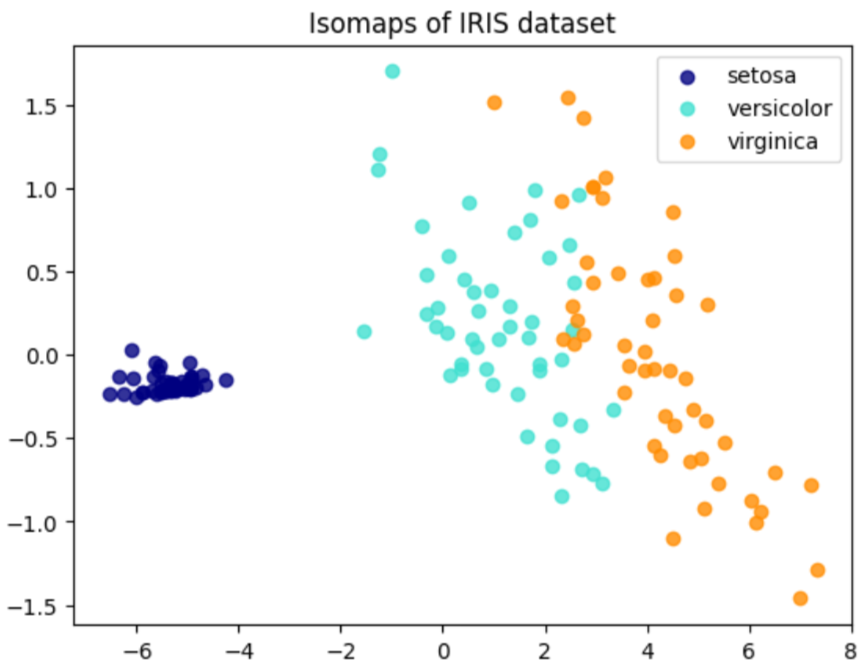
\includegraphics[width=0.5\textwidth]{figures/theory-example-figures/iris-isomap.png}
    \caption{Isomap on iris}
    \label{fig:iris-isomap}
    \end{figure}

On figure \ref{fig:iris-kernelpca} \gls{kpca} has tried to separate the setosa. On the figure it can be seen that \gls{kpca} has clustered the other two species on the first projection, but there cannot be seen any clear separation between the two species, especially on the second projection. \gls{kpca} has also mapped the data points for setosa with a high degree of variance, but it did not clearly separate the setosa from the other two species. Likewise \gls{isomap}, \gls{kpca} was not supposed to separate the data as good as the linear methods, but it is interesting that KernelPCA has not managed to fully separate the setosa species from the rest of the data.

\begin{figure}[htb!]
    \centering
    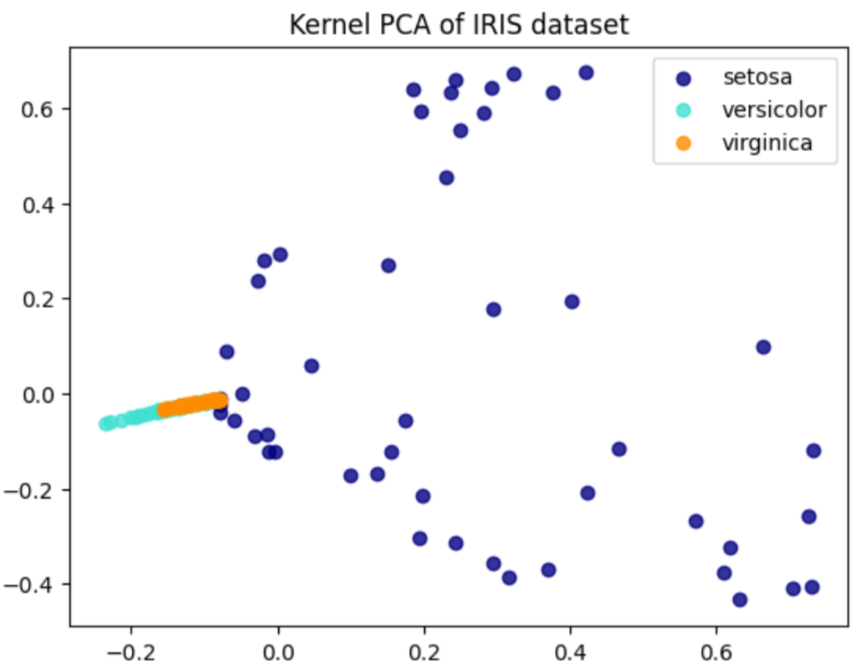
\includegraphics[width=0.5\textwidth]{figures/theory-example-figures/iris-kernelpca.png}
    \caption{KernelPCA on iris}
    \label{fig:iris-kernelpca}
    \end{figure}

\subsection{Nonlinear data example}\label{subsec:nonlinear-data-example}
As nonlinear data we will construct two different classes of cirlces, an inner- and outer circle, which will look like in the figure ~\ref{fig:circles}.

\begin{figure}[htb!]
    \centering
    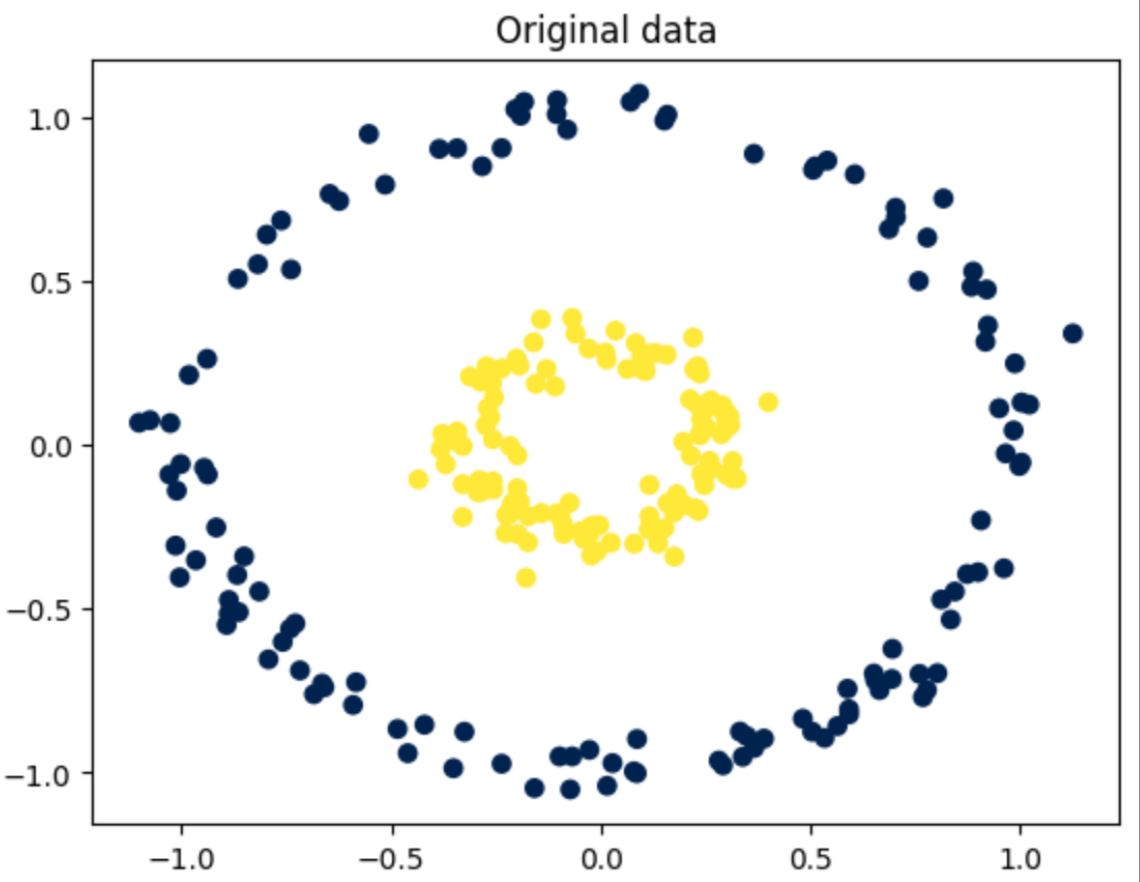
\includegraphics[width=0.5\textwidth]{figures/theory-example-figures/fig-circles.png}
    \caption{Nonlinear data as two circles}
    \label{fig:circles}
    \end{figure}

\subsubsection{Linear methods}\label{subsubsec:linear-methods-on-circles}
\begin{figure}[htb!]
    \centering
    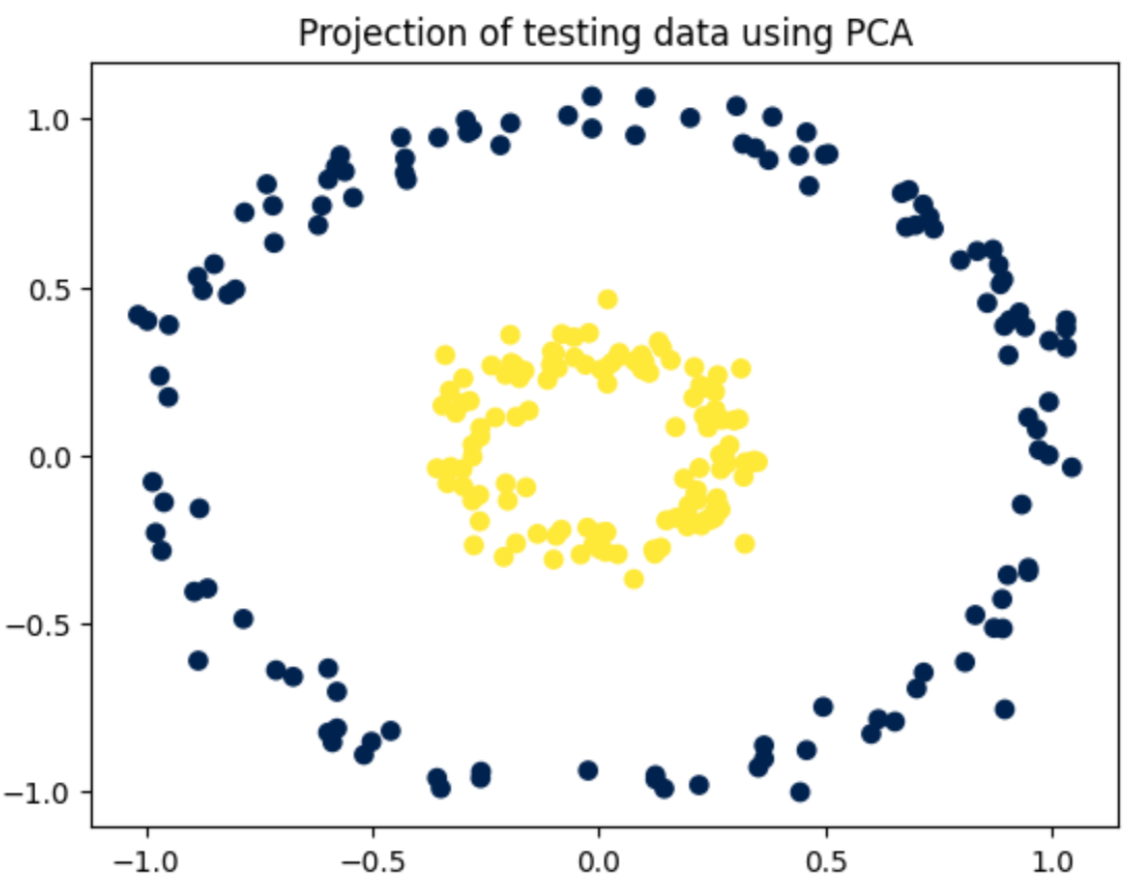
\includegraphics[width=0.5\textwidth]{figures/theory-example-figures/circles-pca.png}
    \caption{PCA on circles}
    \label{fig:circles-pca}
\end{figure}

On figure ~\ref{fig:circles-pca} it can be seen that \gls{pca}'s transformation did not manage to map the nonlinear data at all. On figure \ref{fig:circles-lda} \gls{lda} has reduced the data's dimensions to one dimension, but the two classes are clustered, which means that \gls{lda} could not separate the two classes.

\begin{figure}[htb!]
    \centering
    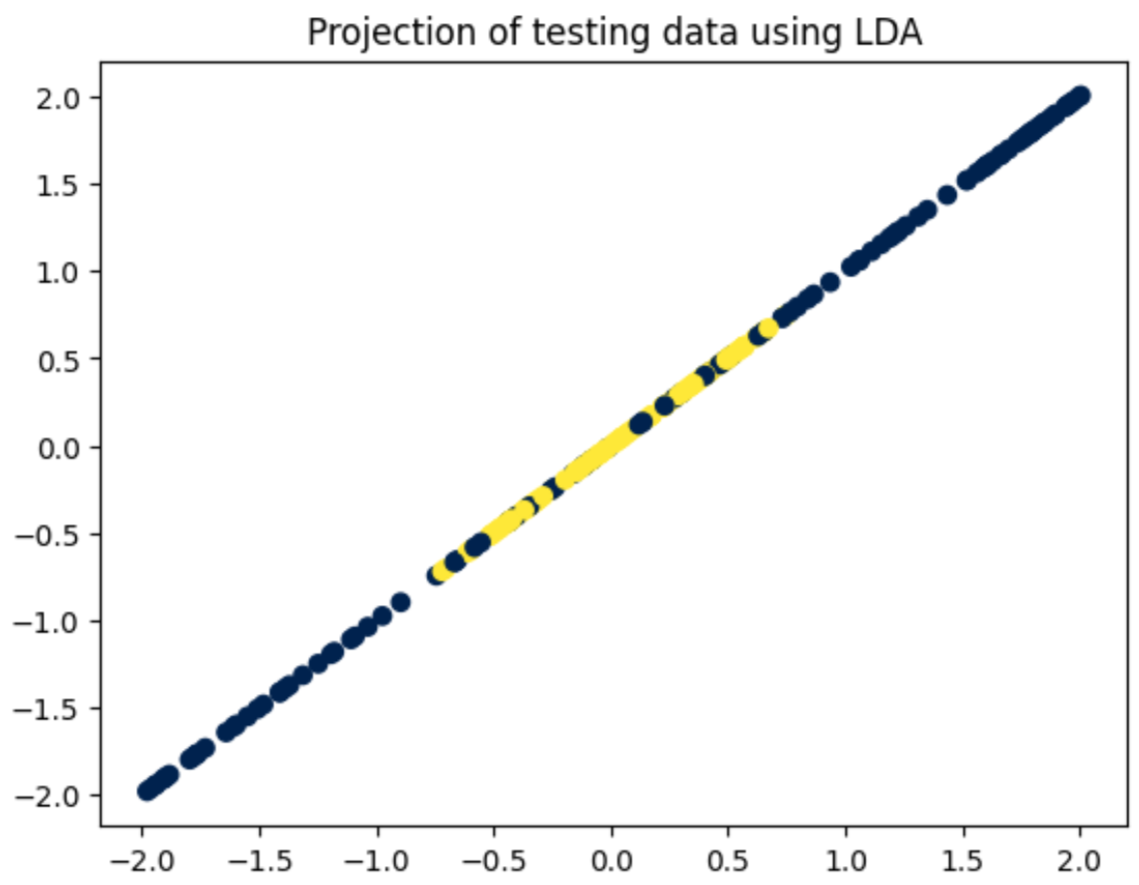
\includegraphics[width=0.5\textwidth]{figures/theory-example-figures/circles-lda.png}
    \caption{LDA on circles}
    \label{fig:circles-lda}
    \end{figure}
    
\subsubsection{Nonlinear methods}\label{subsubsec:nonlinear-methods-on-circles}
On figure \ref{fig:circles-isomap} \gls{isomap} has separated the data points from the circles. Based on the first projection Isomap is capable of separating the data, and on the second projection the method is capable of capturing more information about the outer circle, thus approximating the the original data, as the outer circle has a higher variance than the inner circle. On the second projection \gls{isomap} did not reveal that much information about the inner circle.
\begin{figure}[htb!]
    \centering
    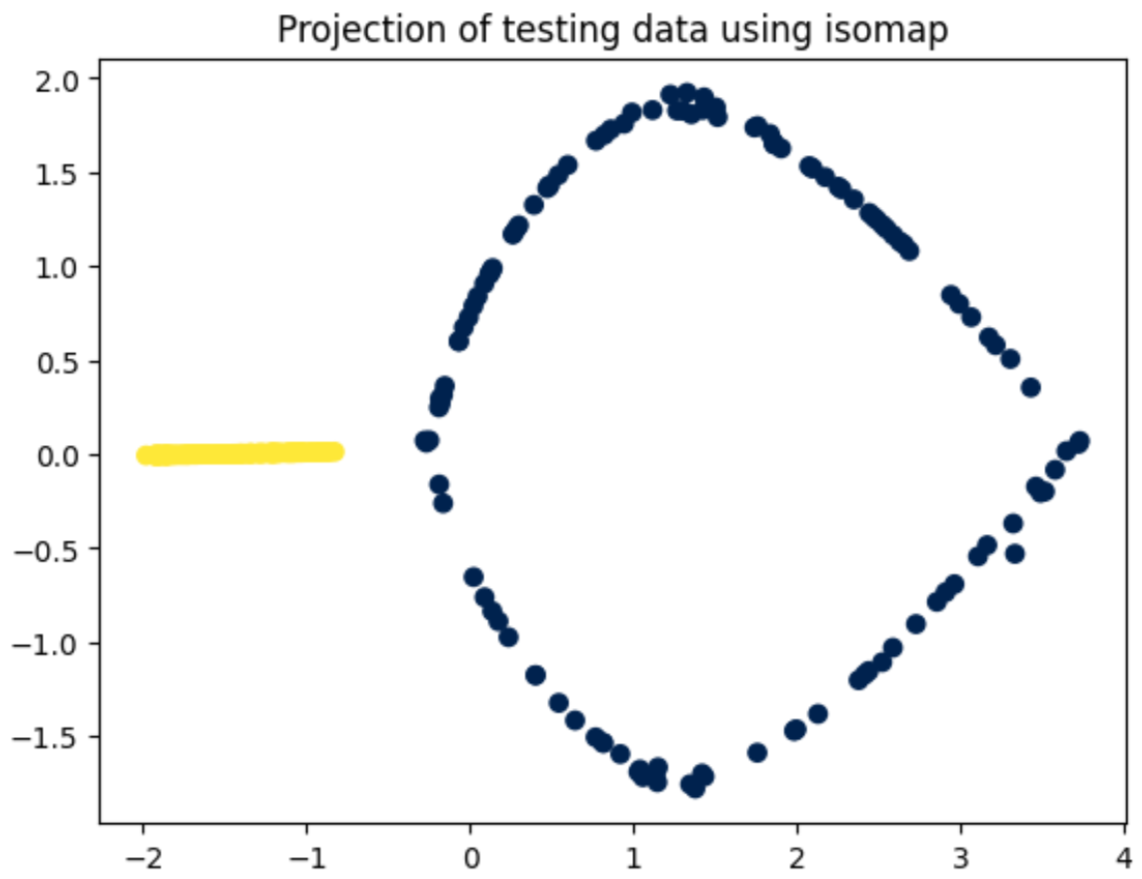
\includegraphics[width=0.5\textwidth]{figures/theory-example-figures/circles-isomap.png}
    \caption{Isomap on circles}
    \label{fig:circles-isomap}
\end{figure}


On figure \ref{fig:circles-kernelpca} \gls{kpca} has also separated the data points from the circles. \gls{kpca} does a good job at maximizing the variance for the inner circle, and also separating the the data points from each other. As it can be seen \gls{kpca} needs at least two dimensions in order to better differentiate between the two classes, as opposed to \gls{isomap}, which only needs one dimension.
\begin{figure}[htb!]
    \centering
    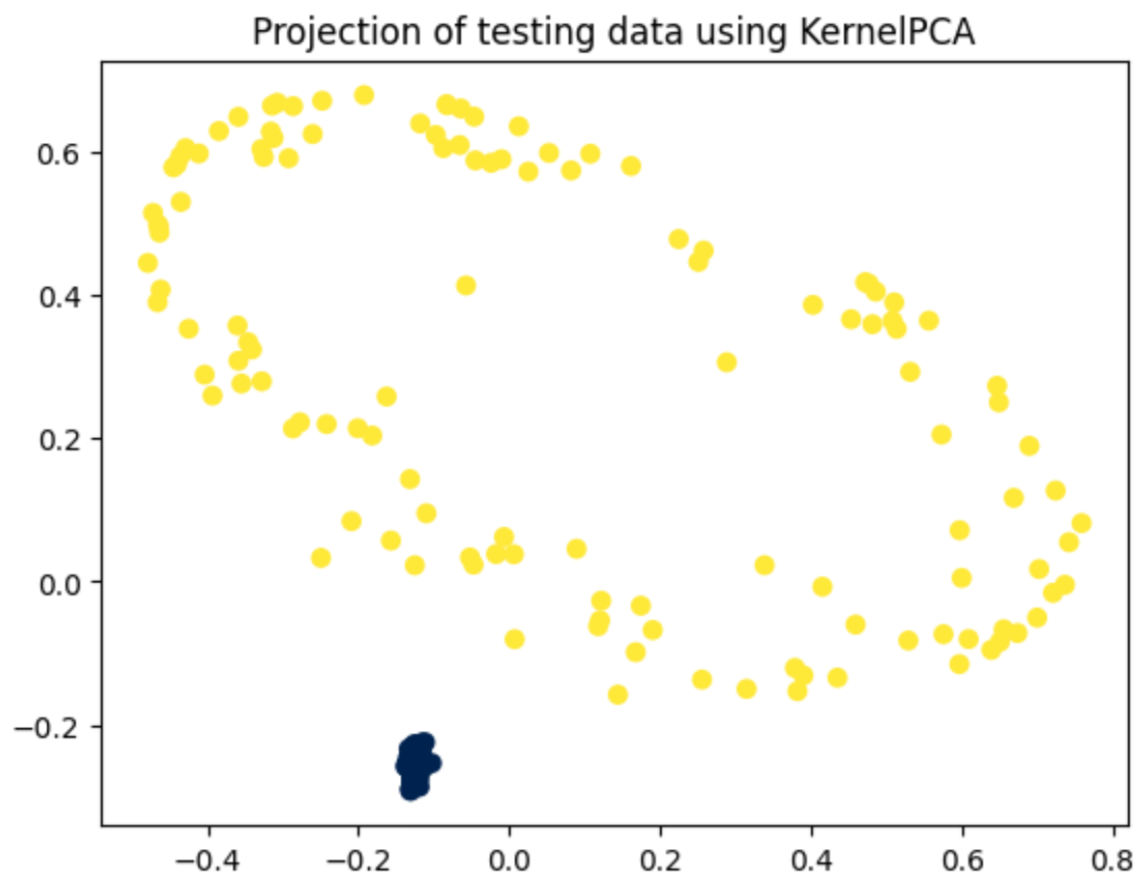
\includegraphics[width=0.5\textwidth]{figures/theory-example-figures/circles-kernelpca.png}
    \caption{KernelPCA on circles}
    \label{fig:circles-kernelpca}
\end{figure}


Until now we have presented some simple examples of the methods. More often than not, the number dimensions reduced will not be two, as there will be much more relevant information in the other dimensions too.

% @misc{iris-dataset,
% author = "Dua, Dheeru and Graff, Casey",
% year = "2017",
% title = "{UCI} Machine Learning Repository",
% url = "http://archive.ics.uci.edu/ml",
% institution = "University of California, Irvine, School of Information and Computer Sciences" }
\section{Hyperparameter optimization}\label{sec:hyperparam}
This section introduces the concept of hyperparameter optimization and the importance of this process in machine learning.


\subsection{Hyperparameters}\label{subsec:hyperparam-what}
Hyperparameters are the parameters set, for algorithms, before training the model, which does not get learned from the data. The values of hyperparameters can have a significant impact on the performance of the model. How hyperparameters differ from model parameters is that those model parameters get learned from the data during model training~\cite{probst2019tunability}.

Hyperparameters exist for both \gls{fe} and for \gls{ml} models, examples of these could be \gls{svm} and \gls{pca}. Here \gls{pca} should at least have the hyperparameter which corresponds to the amount of dimensions it should reduce down to. \gls{svm} would have hyperparameters like which kind of kernel it should use~\cite{probst2019tunability}.

\subsection{Methods of optimization for hyperparameters}\label{subsec:hyperparam-how}
Usually, when selecting hyperparameters for a given algorithm, users can resort to default values based on the algorithm's documentation, read literature for recommendations, or try different values and see which one works best. However, this approach could be more efficient, as it is time-consuming and requires a lot of manual work~\cite{probst2019tunability}.

Instead, the process of finding optimal hyperparameters can be given to the computer~\cite{automated-machine-learning}, given a set of configurations. Hyperparameter optimization is complex because it is unknown which hyperparameters will significantly affect the model, which hyperparameters will interact with each other, and how their interactions will change the model's performance. According to Marc Claesen~\cite{hyperparam-search}, the number of hyperparameters that have a significant impact may be small, but that does not mean that the number of meaningful combinations may be small too.

Many different techniques can get used to optimize the hyperparameters automatically~\cite{automated-machine-learning}. An example of such a technique is grid search. This technique allows the user to define \textcquote{automated-machine-learning}{a set of finite values for each hyperparameter, and grid search evaluates the Cartesian product of these sets}.

Another example of a method is random search, a technique similar to grid search. However, instead of evaluating all the combinations of hyperparameters, it randomly evaluates hyperparameters, given a limited amount of time. Both methods have limitations; grid search is inefficient when the number of hyperparameters is significant due to the curse of dimensionality, which means that for algorithms that require large amounts of hyperparameters, it is not feasible to use this technique~\cite{yang2020hyperparameter}.

Random search can prove helpful, but there is no guarantee that it will find the optimal hyperparameters, given its limited time to evaluate them. Knowing the optimal time limit for random search is tricky, as it depends on the number of hyperparameters, the number of possible values for each hyperparameter, and the number of times the hyperparameters are evaluated~\cite{yang2020hyperparameter}.

From this, it can be concluded that no single method is optimal for all cases. The optimal method depends on many variables, such as the number of hyperparameters and possible values for each hyperparameter. Therefore, it is essential to evaluate the different methods and find the one that works best for the given problem. Of course, many other techniques could be discussed. Nevertheless, these two methods should sufficiently demonstrate the strengths and weaknesses of different techniques.

\subsection{Choice of hyperparameter tuning}
Choosing parameters is necessary when working with models and with \gls{fe}. In this pipeline, in particular, there are many parameters to tune because it has both model and \gls{fe}. Tuning the parameters would take very long due to not only having to pick different model parameters and try each of these configurations with different \gls{fe}, which increases the time exponentially.

The pipeline implements hyperparameter tuning, specifically using grid search to solve this. This hyperparameter tuning using grid search makes the tuning process more effective and avoids missing exemplary configurations due to human error.

\section{Cross-validation}\label{sec:cross-validation}

This section will describe cross-validation, why it is used in general and why it is used in this project.

A common problem in machine learning is that the test set is supposed to be used only in the final evaluation. This problem makes it hard to, for example, hyperparameter tune or chooses the correct model for the data. On the other hand, if the test data is used to tune or choose a model, this often leads to overfitting ~\cite{james-statistical-learning}.
Overfitting can be described as when the model is very good at predicting the test data but will not do well with new data, not from the test set. This section will introduce one technique that will reduce the chances of overfitting the model: cross-validation. Cross-validation is a technique that splits the data into three sets: training data, validation data(comprising of training data), and test data. By partitioning the training data into two sets, the model can learn from the training data and evaluate on the validation data. The model can be tuned with the validation data and evaluated on the test data after the model is optimized. Such an approach is practical because the model gets evaluated based on data it has never seen, which shows how good the model is at predicting data it has not yet seen ~\cite{scikit-learn-ml}. Cross-validation is particularly useful with hyperparameter tuning because it allows picking the correct parameters without using the test set.


Cross-validation, more practically can be described as \textcquote{Refaeilzadeh2009}
{The basic form of cross-validation is the basic form of k-fold cross-validation. (. . .) In k-fold cross-validation, the data is first partitioned into $k$ equally (or nearly equally) sized segments or folds. Subsequently, $k$ iterations of training and validation are performed such that within each iteration a different fold of the data is held-out for validation while the remaining $k-1$ folds are used for learning.}

There are also exists other forms of cross-validation, which are special cases of k-fold. As described before, shuffling the data might be necessary, and there is a version of k-fold called Stratified k-fold, where the data gets reshuffled for each round. Alternatively, instead of shuffling the data, one can use the leave-one-out cross-validation, where for each fold, all of the data except one sample is used for training ~\cite{Refaeilzadeh2009}. Stratifying or shuffling the data may be necessary so that each fold has a balanced distribution of classes. There is a risk that the folds contain imbalanced samples for each class, which may affect the overall model performance because the model is biased towards the majority class ~\cite{Refaeilzadeh2009}.

In order to avoid overfitting, one can use k-fold cross-validation or derivatives of it, but k-fold implies that a specific number must be chosen. The choice of $k$ could be made through trial and error. However, the train and data samples need to be large enough to be statistically representative of the data set ~\cite{Refaeilzadeh2009}.
\section{Evaluation and metrics}\label{sec:evalueation}

A pipeline is generally evaluated based on quantitative metrics in machine learning and data science. These metrics are in classification general based on the confusion matrix. An example of a confusion matrix can be seen in \todo{need to make pictue}. It represents all the guesses a ml model has made, where the x-axis, in this case, is the true class of a given data point, and the y-axis is the class the model has guessed the data point to have. The numbers are how many times the model has guessed the different combinations. \cite{james-statistical-learning}

\subsection*{Metrics}

There exist many metrics, but generally, there are four basic metrics. These are accuracy, precision, recall, and f1. Outside these, there are more esoteric metrics like the Mattheus correlation coefficient, Cohen's kappa, and more. The following section will describe each of the four basic metrics. \cite{metrics-for-multi}

Accuracy is the most straightforward of the metrics. It describes the percentage of correct guesses out of all guesses. This metric works well in cases where the sizes of the different classes are similar. It struggles in cases where one class is much larger than another. Here It is possible to achieve very high accuracy by only guessing the larger class, which can make a model seem impressive while simultaneously not doing what it is supposed to if it is crucial to find the smaller class.

In the case where one class is smaller is where the precision metric comes in handy. It is calculated by taking the correct guesses for a class and dividing them by all guesses on this class, which includes wrong guesses. This gets around the problems accuracy has with classes with very different sizes because it is not possible to always guess the bigger class and get a good precision.

The third metric is recall, primarily used in cases where it really matters if one class is guessed correctly. Recall could be in cases like corona, where a false positive is much better than a false negative. Recall is calculated by dividing the true positives by true positives and false negatives.

The last basic metric is f1. Its commonly used when both recall and precision are essential. It is calculated two times precision times recall decided by precision plus recall.


In a pipeline, these metrics are generally used for hyperparameter tuning and general evaluation of the model's performance. Here hyperparameter tuning will generally only use a single metric to focus on to maximize it. In evaluation, on the other hand, the metrics are used more generally to explain what the model does well and what it does not do well. \cite{james-statistical-learning}